%%
%% This is file `sample-sigplan.tex',
%% generated with the docstrip utility.
%%
%% The original source files were:
%%
%% samples.dtx  (with options: `sigplan')
%%
%% IMPORTANT NOTICE:
%%
%% For the copyright see the source file.
%%
%% Any modified versions of this file must be renamed
%% with new filenames distinct from sample-sigplan.tex.
%%
%% For distribution of the original source see the terms
%% for copying and modification in the file samples.dtx.
%%
%% This generated file may be distributed as long as the
%% original source files, as listed above, are part of the
%% same distribution. (The sources need not necessarily be
%% in the same archive or directory.)
%%
%%
%% Commands for TeXCount
%TC:macro \cite [option:text,text]
%TC:macro \citep [option:text,text]
%TC:macro \citet [option:text,text]
%TC:envir table 0 1
%TC:envir table* 0 1
%TC:envir tabular [ignore] word
%TC:envir displaymath 0 word
%TC:envir math 0 word
%TC:envir comment 0 0
%%
%%
%% The first command in your LaTeX source must be the \documentclass command.
%%\documentclass[sigplan,nonacm]{acmart}
\documentclass[sigplan,screen,nonacm]{acmart}\settopmatter{printfolios=true,printccs=false,printacmref=false}
\graphicspath{{figure/}}
%%
%% \BibTeX command to typeset BibTeX logo in the docs
\AtBeginDocument{%
	\providecommand\BibTeX{{%
			\normalfont B\kern-0.5em{\scshape i\kern-0.25em b}\kern-0.8em\TeX}}}

%% Rights management information.  This information is sent to you
%% when you complete the rights form.  These commands have SAMPLE
%% values in them; it is your responsibility as an author to replace
%% the commands and values with those provided to you when you
%% complete the rights form.
\setcopyright{none}

%%\copyrightyear{2018}
%%\acmYear{2018}
%%\acmDOI{10.1145/1122445.1122456}

%% These commands are for a PROCEEDINGS abstract or paper.
%%\acmConference[Woodstock '18]{Woodstock '18: ACM Symposium%% on Neural
%%  Gaze Detection}{June 03--05, 2018}{Woodstock, NY}
%%\acmBooktitle{Woodstock '18: ACM Symposium on Neural Gaze Detection,
%%  June 03--05, 2018, Woodstock, NY}
%%\acmPrice{15.00}
%%\acmISBN{978-1-4503-XXXX-X/18/06}


%%
%% Submission ID.
%% Use this when submitting an article to a sponsored event. You'll
%% receive a unique submission ID from the organizers
%% of the event, and this ID should be used as the parameter to this command.
%%\acmSubmissionID{123-A56-BU3}

%%
%% The majority of ACM publications use numbered citations and
%% references.  The command \citestyle{authoryear} switches to the
%% "author year" style.
%%
%% If you are preparing content for an event
%% sponsored by ACM SIGGRAPH, you must use the "author year" style of
%% citations and references.
%% Uncommenting
%% the next command will enable that style.
%%\citestyle{acmauthoryear}

%%
%% end of the preamble, start of the body of the document source.
\begin{document}
\sloppy

%%
%% The "title" command has an optional parameter,
%% allowing the author to define a "short title" to be used in page headers.
\title{A brief study of Approximation Algorithms for 2D Packing Problem}

%%
%% The "author" command and its associated commands are used to define
%% the authors and their affiliations.
%% Of note is the shared affiliation of the first two authors, and the
%% "authornote" and "authornotemark" commands
%% used to denote shared contribution to the research.
\author{Ruiqi Gao}
\email{gao606@purdue.edu}
\affiliation{%
  \institution{Purdue University}
  \city{Lafayette}
  \state{Indiana}
  \country{USA}
  \postcode{47901}
}



%%
%% By default, the full list of authors will be used in the page
%% headers. Often, this list is too long, and will overlap
%% other information printed in the page headers. This command allows
%% the author to define a more concise list
%% of authors' names for this purpose.
%%\renewcommand{\shortauthors}{Trovato and Tobin, et al.}

%%
%% The abstract is a short summary of the work to be presented in the
%% article.
\begin{abstract}
  2D Packing Problem (Strip Packing) is a 2-dimensional minimization geometric optimization problem where we pack a rectangles into a unit-width bin with infinite height to minimize the packing height. In this paper we study a series of approximation algorithm for 2D Packing Problem, analyze the performance. First we will study the 2 early stage intuitive approximation algorithm designed by Coffman with approximation bound 3 and 2.7. Then we will further investigate a more advanced algorithm designed by Steinberg that have a approximation bound of 2. We will also explore some future direction of this problem in the end.
\end{abstract}
\keywords{Approximation Algorithm, 2D packing, Strip Packing}

%%
%% The code below is generated by the tool at http://dl.acm.org/ccs.cfm.
%% Please copy and paste the code instead of the example below.
%%


%%
%% Keywords. The author(s) should pick words that accurately describe
%% the work being presented. Separate the keywords with commas.



%%
%% This command processes the author and affiliation and title
%% information and builds the first part of the formatted document.
\maketitle

\section{Introduction}
2D Packing Problem is defined as follows: We are giving a collection of rectangles $\{R_1,R_2,R_3,\dots,R_n\}$ and a bin with fixed width and infinite height, and we need to pack all the rectangles into the bin without overlapping while minimize the total bin height\cite{baker1980orthogonal}. Without loss of generality, we can normalize the width to be 1.\par
\begin{figure}[htbp]
  \centering
  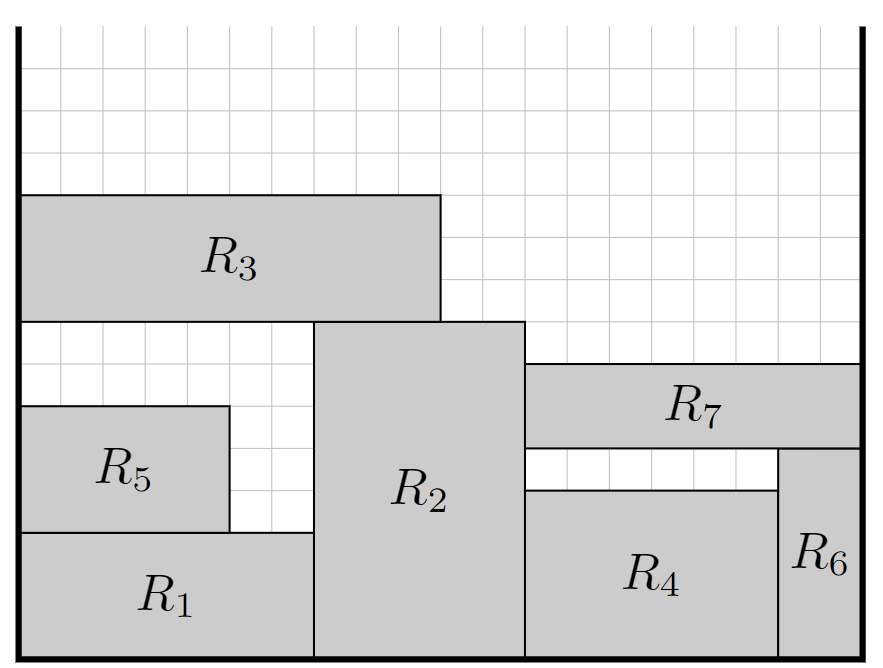
\includegraphics[scale=0.5]{2dpacking}
  \caption{2D Packing Problem}
  \label{fig:2dpacking}
\end{figure}
This problem is very important in many fields. In transportation industry, this algorithm can be used to pack item into containers. There is also an interesting application of this problem in main memory allocation in multi processor programming. Basically, this problem can be adopted to most resource allocation problem with two dimension resource constraints.\par
While the description of this problem is rather simple, there is a hidden computation complexity behind this problem. Actually, this problem is NP-Complete\cite{hartmanis1982computers}, which means that there is currently no efficient deterministic algorithm to solve it. It is easy to notice that this problem is a generalized version of one-dimension bin packing problem\cite{johnson1974worst}. Simply restrict all the rectangles' height to be 1, this problem becomes one-dimensional bin packing problem. We can reduce the one-dimensional bin packing problem to this problem using the idea above. Because one-dimensional bin packing problem is NP-Hard, this problem is also NP-Hard. The optimized solution to 2D Packing problem can be easily verified, therefore 2D Packing Problem is also in NP. Then 2D Packing Problem is NP-Complete. With $P$ $vs$ $NP$ being an open problem, we can not find an efficient algorithm for 2D Packing Problem. \par
Another interesting NP-Complete problem that is related to 2D Packing is MakeSpan minimization problem\cite{graham1966bounds} where we try to schedule jobs across multiple machines and minimize the total execution time. By simply restricting all the rectangles' height to be 1, 2D Packing Problem becomes MakeSpan minimization problem. By finding an efficient algorithm for 2D Packing Problem, we can find an efficient solution to MakeSpan minimization problem too. \par
We already show that 2D Packing Problem to be NP-Complete, and P vs NP remains an open problem, so we can not find an efficient algorithm to deterministically solve it. We must try other approach. To solve inherently difficult problem, various approach have been well-studied. For decision problem, we can use randomized algorithm to give the correct result with high probability. For optimization problem, we can use another approach: Approximation algorithm\cite{garey1976approximation} which is guaranteed to produce a sub-optimal but reasonable result. \par
In this paper, we are going to investigate various approximation algorithm for 2D Packing Algorithm. In section 2, we will brief study the definition and performance metric for Approximation algorithms. In section 3, we will introduce two early level-oriented heuristic approximation algorithm\cite{coffman1980performance} for 2D Packing Problem. In section 4,  we will study a more advanced approach\cite{steinberg1997strip}.
\section{Approximation Algorithm}
For inherently difficult problems like NP-Complete problems, various approaches have been well-studied to efficiently solve them. The most common approach to solve an optimization problem is Approximation algorithm. Approximation algorithm aims to find an approximate solution to the optimal solution, then we can efficient solve the target problem with a tight performance bounds using approximation algorithm.\par
The analysis for Approximation algorithm often requires a through mathematical proof for the worst case performance. We can find some surprising properties for hard problems through Approximation algorithms. Although all NP-Complete problems are equivalently difficult, their complexity varies in the perspective of Approximation algorithm. For example, knapsack can produce solutions that is arbitrarily close to the optimal result. However, finding a solution that is constant-bounded to the optimal result for Maximum clique problem is proved to be equivalent to prove whether P = NP. Therefore, Algorithm provided a extra classification for NP-hard problems.\par
Now we are going to look at the performance metrics for Approximation algorithms.
\subsection{Approximation Ratio}
To measure the performance of approximation, we need to quantify the difference between produced result and the optimal solution. The most commonly used metrics is the multiplicative factor between the solution and the optimum. For problem $L$, assume that the algorithm is $A$, the optimal result is $OPT(L)$, the produced solution is $A(L)$:
$$R(A) = max(\frac{OPT(L)}{A(L)}, \frac{A(L)}{OPT(L)})$$
Then for minimization problem, approximation ratio $\alpha$ puts a multiplicative maximum bound on the result $A(L) \leq \alpha*OPT(L)$. For maximization, approximation ratio puts a multiplicative minimum bound on the result $A(L) \geq \frac{OPT(L)}{\alpha}$. We can also call this ratio Absolute Approximation Ratios to be precise.
\subsection{Asymptotic Approximation Ratio}
Different from Approximation ratio that only uses an multiplicative bound factor, Asymptotic Approximation use an additional additive bound factor. This gives us a more fine-grained metric to measure the performance of Approximation algorithm. For minimization problem, an Asymptotic bound $\alpha$ means that:
$$ A(L) \leq \alpha*OPT(L) + \gamma $$
$\gamma$ is a additive constant factor. It should be noticed that any asymptotic approximation ratio can be relaxed into a weaker absolute approximation bound.\par
After we introduce different metric for measuring the performance of approximation algorithm, we will show how to analyze approximation algorithm using this metrics in the next section with 2 intuitive algorithm for 2D Packing.
\section{Early Approximation Algorithm for 2D Packing}
In this section we are going to look at some 2 dimensional analogue of the one-dimensional approximation packing algorithms\cite{johnson1974worst}-NFDH and FFDH algorithms. NFDH has an asymptotic approximation ratio of 2 and absolute approximation ratio 3. FFDH has a tighter asymptotic approximation ratios of 1.7 and a corresponding absolute approximation ratio 2.7. We are also going to see the proof of these approximation ratios and gain some insight into the analysis for approximation algorithm.\par
Both NFDH (Next-Fit Decreasing-Height) and FFDH (First-Fit Decreasing-Height) algorithms are level-based\ref{fig:level-based}, which means that the packing will be a sequence of levels. Each level are horizontal lines on top of the highest rectangle from previous level and the first level is simply the bottom of the bin. All the rectangles must place their bottoms on one of these levels. So rectangles can not be placed on top of each other inside each level.
\begin{figure}[htbp]
  \centering
  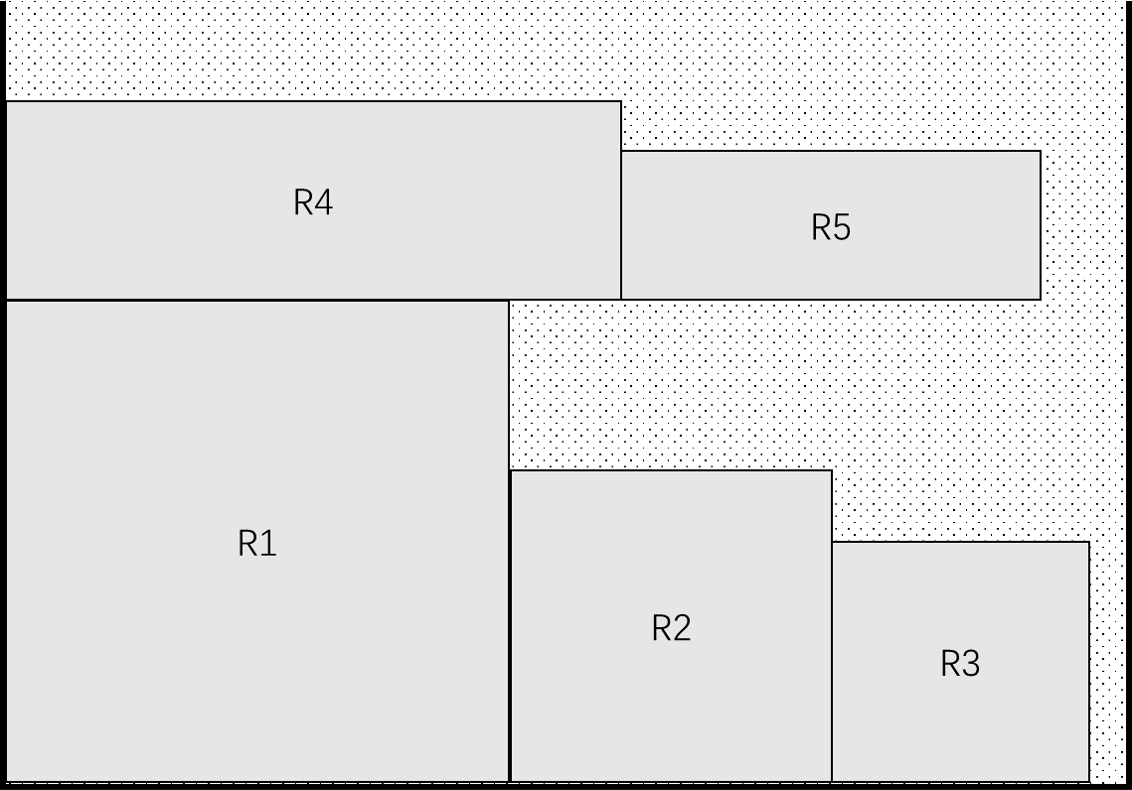
\includegraphics[scale=0.4]{levelbased}
  \caption{Level-Based Packing}
  \label{fig:level-based}
\end{figure}
At first glance, this level-based approach seems to wasteful because the space between level and the rectangle below it is not used. One might think that by putting the rectangle at the lowest-possible place we can achieve a much better result. But as we will show later in the analysis, this new approach will only reduces an additive constant factor which will not affect the algorithm's asymptotic approximation ratio.\par
NFDH and FFDH both are two dimensional variation of the one-dimensional packing algorithm\cite{johnson1974worst}. They all have a preprocessing procedure to sort all the rectangles with decreasing height. We will introduce both of the 2 algorithm and analyze their approximation ratio in the following subsections.
\subsection{NFDH (Next-Fit Decreasing-Height)}
\paragraph*{Algorithm Description}
NFDH proceed as follows: After we sort all the rectangles with decreasing height. We simply pack rectangles left-justified from left to right on the bottom of the bin (the first level), so the first rectangle is the highest rectangle. When there is no more sufficient width in the current level, we proceed to the next level (a horizontal line on top of the first rectangle in the current level). We just iterate from level to level until we pack all the rectangles.
\paragraph{Performance Analysis}
It may seem that we are wasting a large number of space by using the level-based NFDH algorithm, but NFDH has an asymptotic approximation ratio of 2 and an absolute approximation ratio of 3 ($h_{max}$ is the maximum height of all the rectangles).
$$NFDH(L) \leq 2*OPT(L) + h_{max}$$
The analysis is shown below.\par

\subsection{FFDH (First-Fit Decreasing-Height)}
\bibliographystyle{acm}
\bibliography{paper}
\end{document}
\endinput
